\documentclass[12pt,a4paper]{article}
\usepackage[margin=1in]{geometry}
\usepackage{amsmath,amssymb,amsfonts}
\usepackage{graphicx}
\usepackage{hyperref}
\usepackage{listings}
\usepackage{xcolor}
\usepackage{booktabs}
\usepackage{longtable}
\usepackage{array}
\usepackage{multirow}
\usepackage{tikz}
\usetikzlibrary{shapes,arrows,positioning,fit,calc}
\usepackage{float}
\usepackage{enumitem}
\usepackage{fancyhdr}
\usepackage{tcolorbox}

\pagestyle{fancy}
\fancyhf{}
\rhead{CA Lab 3 -- Theory Document (Part 3)}
\lhead{ToyRISC Simulator Architecture}
\cfoot{\thepage}

\definecolor{codegreen}{rgb}{0,0.6,0}
\definecolor{codegray}{rgb}{0.5,0.5,0.5}
\definecolor{codepurple}{rgb}{0.58,0,0.82}
\definecolor{backcolour}{rgb}{0.95,0.95,0.92}

\lstdefinestyle{javastyle}{
    backgroundcolor=\color{backcolour},
    commentstyle=\color{codegreen},
    keywordstyle=\color{blue}\bfseries,
    numberstyle=\tiny\color{codegray},
    stringstyle=\color{codepurple},
    basicstyle=\ttfamily\footnotesize,
    breakatwhitespace=false,
    breaklines=true,
    captionpos=b,
    keepspaces=true,
    numbers=left,
    numbersep=5pt,
    showspaces=false,
    showstringspaces=false,
    showtabs=false,
    tabsize=2,
    frame=single
}

\lstdefinestyle{asmstyle}{
    backgroundcolor=\color{backcolour},
    commentstyle=\color{codegreen},
    keywordstyle=\color{blue}\bfseries,
    basicstyle=\ttfamily\footnotesize,
    breaklines=true,
    captionpos=b,
    keepspaces=true,
    numbers=left,
    numbersep=5pt,
    frame=single,
    morekeywords={add,addi,sub,subi,mul,muli,div,divi,and,andi,or,ori,xor,xori,slt,slti,sll,slli,srl,srli,sra,srai,load,store,jmp,beq,bne,blt,bgt,end}
}

\title{\Huge\bfseries Comprehensive Theory of Single-Cycle Processor Design and the ToyRISC ISA\\[1em]
\Large Part 3: Simulator Architecture, Code Walkthrough, and Test Programs}
\author{Computer Architecture Laboratory -- Assignment 3}
\date{\today}

\begin{document}

\maketitle
\tableofcontents
\newpage

% ===========================================================================
\section{Simulator Architecture Overview}
% ===========================================================================

The ToyRISC simulator is a Java-based architectural simulator that models a single-cycle processor. It is organized into four packages reflecting a clean separation of concerns.

\subsection{Package Structure}

\begin{figure}[H]
\centering
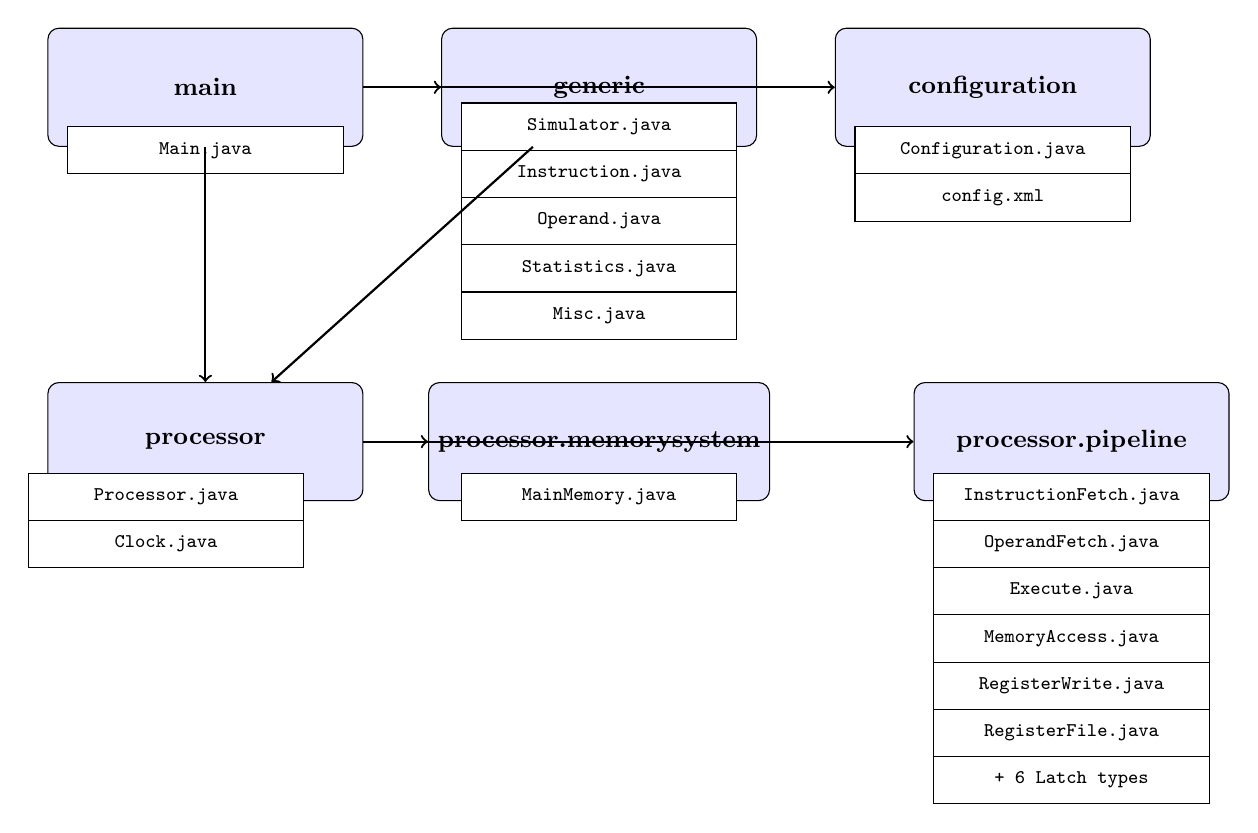
\begin{tikzpicture}[
    package/.style={draw, rectangle, rounded corners, minimum width=4cm, minimum height=1.5cm, text centered, font=\bfseries\small, fill=blue!10},
    file/.style={draw, rectangle, minimum width=3.5cm, minimum height=0.6cm, text centered, font=\ttfamily\scriptsize, fill=white},
    arrow/.style={->, thick}
]
\node[package] (main) at (0,6) {main};
\node[file] at (0,5.2) {Main.java};

\node[package] (generic) at (5,6) {generic};
\node[file] at (5,5.5) {Simulator.java};
\node[file] at (5,4.9) {Instruction.java};
\node[file] at (5,4.3) {Operand.java};
\node[file] at (5,3.7) {Statistics.java};
\node[file] at (5,3.1) {Misc.java};

\node[package] (config) at (10,6) {configuration};
\node[file] at (10,5.2) {Configuration.java};
\node[file] at (10,4.6) {config.xml};

\node[package] (proc) at (0,1.5) {processor};
\node[file] at (-0.5,0.8) {Processor.java};
\node[file] at (-0.5,0.2) {Clock.java};

\node[package] (mem) at (5,1.5) {processor.memorysystem};
\node[file] at (5,0.8) {MainMemory.java};

\node[package] (pipe) at (11,1.5) {processor.pipeline};
\node[file] at (11,0.8) {InstructionFetch.java};
\node[file] at (11,0.2) {OperandFetch.java};
\node[file] at (11,-0.4) {Execute.java};
\node[file] at (11,-1.0) {MemoryAccess.java};
\node[file] at (11,-1.6) {RegisterWrite.java};
\node[file] at (11,-2.2) {RegisterFile.java};
\node[file] at (11,-2.8) {+ 6 Latch types};

\draw[arrow] (main) -- (generic);
\draw[arrow] (main) -- (config);
\draw[arrow] (main) -- (proc);
\draw[arrow] (generic) -- (proc);
\draw[arrow] (proc) -- (mem);
\draw[arrow] (proc) -- (pipe);
\end{tikzpicture}
\caption{Package dependency diagram}
\end{figure}

\subsection{Execution Flow}

The program execution follows this sequence:

\begin{enumerate}
    \item \texttt{Main.main()} parses command-line arguments (config file, stats file, object file).
    \item \texttt{Configuration.parseConfigurationFile()} reads processor parameters from XML.
    \item A \texttt{Processor} object is created, which instantiates all pipeline stages, latches, register file, and memory.
    \item \texttt{Simulator.setupSimulation()} loads the object file into memory and initializes registers.
    \item \texttt{Simulator.simulate()} runs the main simulation loop: IF $\to$ OF $\to$ EX $\to$ MA $\to$ RW, repeating until \texttt{end} is encountered.
    \item Final processor state is printed (registers and memory).
    \item Statistics are written to the output file.
    \item A hash of the final processor state is computed and printed (for verification).
\end{enumerate}

% ===========================================================================
\section{Detailed Code Walkthrough}
% ===========================================================================

\subsection{Main.java -- Entry Point}

\begin{lstlisting}[style=javastyle, caption={Main.java}]
public class Main {
    public static void main(String[] args) {
        // args[0] = config file path
        // args[1] = statistics output file path
        // args[2] = object file path

        Configuration.parseConfiguratioFile(args[0]);
        Processor processor = new Processor();

        Simulator.setupSimulation(args[2], processor);
        Simulator.simulate();

        processor.printState(0, 30);
        Statistics.printStatistics(args[1]);

        System.out.println("Hash of the Processor State = "
            + getHashCode(processor.getRegisterFile(),
                          processor.getMainMemory()));
    }

    static int getHashCode(RegisterFile regState,
                           MainMemory memState) {
        ArrayList<Integer> hash = new ArrayList<>();
        hash.add(regState.getProgramCounter());
        for (int i = 0; i < 32; i++)
            hash.add(regState.getValue(i));
        for (int i = 0; i < 65536; i++)
            hash.add(memState.getWord(i));
        return hash.hashCode();
    }
}
\end{lstlisting}

\textbf{Key Points}:
\begin{itemize}
    \item The hash function incorporates the \textbf{entire processor state}: PC, all 32 registers, and all 65536 memory words. This ensures correctness verification is comprehensive.
    \item The hash uses Java's \texttt{ArrayList.hashCode()}, which computes a deterministic hash based on all elements.
\end{itemize}

\subsection{Processor.java -- The Processor Model}

The \texttt{Processor} class is the central coordinator. It owns all hardware components and wires them together.

\begin{lstlisting}[style=javastyle, caption={Processor.java -- Constructor}]
public class Processor {
    RegisterFile registerFile;
    MainMemory mainMemory;

    // Inter-stage latches
    IF_EnableLatchType IF_EnableLatch;
    IF_OF_LatchType IF_OF_Latch;
    OF_EX_LatchType OF_EX_Latch;
    EX_MA_LatchType EX_MA_Latch;
    EX_IF_LatchType EX_IF_Latch;  // feedback latch
    MA_RW_LatchType MA_RW_Latch;

    // Pipeline stages
    InstructionFetch IFUnit;
    OperandFetch OFUnit;
    Execute EXUnit;
    MemoryAccess MAUnit;
    RegisterWrite RWUnit;

    public Processor() {
        registerFile = new RegisterFile();
        mainMemory = new MainMemory();

        // Create latches
        IF_EnableLatch = new IF_EnableLatchType();
        IF_OF_Latch = new IF_OF_LatchType();
        OF_EX_Latch = new OF_EX_LatchType();
        EX_MA_Latch = new EX_MA_LatchType();
        EX_IF_Latch = new EX_IF_LatchType();
        MA_RW_Latch = new MA_RW_LatchType();

        // Create stages, passing shared latches
        IFUnit = new InstructionFetch(this,
            IF_EnableLatch, IF_OF_Latch, EX_IF_Latch);
        OFUnit = new OperandFetch(this,
            IF_OF_Latch, OF_EX_Latch);
        EXUnit = new Execute(this,
            OF_EX_Latch, EX_MA_Latch, EX_IF_Latch);
        MAUnit = new MemoryAccess(this,
            EX_MA_Latch, MA_RW_Latch);
        RWUnit = new RegisterWrite(this,
            MA_RW_Latch, IF_EnableLatch);
    }
}
\end{lstlisting}

\textbf{Design Pattern -- Dependency Injection}: Each pipeline stage receives references to its input and output latches through the constructor. This is a form of dependency injection that:
\begin{itemize}
    \item Decouples stages from each other (no stage directly references another stage).
    \item Makes the data flow explicit (each stage knows only about its latches).
    \item Facilitates testing (stages can be tested independently with mock latches).
\end{itemize}

\textbf{The EX\_IF Feedback Latch}: Notice that the \texttt{EX\_IF\_Latch} connects the Execute stage back to the Instruction Fetch stage. This is essential for control flow instructions (branches and jumps) that need to redirect the PC.

\subsection{Simulator.java -- Simulation Control}

\begin{lstlisting}[style=javastyle, caption={Simulator.java}]
public class Simulator {
    static Processor processor;
    static boolean simulationComplete;

    public static void setupSimulation(String objFile,
                                       Processor p) {
        Simulator.processor = p;
        loadProgram(objFile);
        simulationComplete = false;
    }

    static void loadProgram(String objFile) {
        // TODO: Load object file into memory
        // 1. Read first int = PC
        // 2. Read remaining ints into memory[0], memory[1], ...
        // 3. Set PC, x0=0, x1=65535, x2=65535
    }

    public static void simulate() {
        while (simulationComplete == false) {
            processor.getIFUnit().performIF();
            Clock.incrementClock();
            processor.getOFUnit().performOF();
            Clock.incrementClock();
            processor.getEXUnit().performEX();
            Clock.incrementClock();
            processor.getMAUnit().performMA();
            Clock.incrementClock();
            processor.getRWUnit().performRW();
            Clock.incrementClock();
        }
        // TODO: Set statistics
    }
}
\end{lstlisting}

\textbf{Simulation Loop Analysis}:
\begin{itemize}
    \item Each iteration processes \textbf{one complete instruction} through all 5 stages.
    \item The clock increments 5 times per instruction (once per stage).
    \item Total cycles = 5 $\times$ number of instructions executed.
    \item The loop terminates when \texttt{simulationComplete} is set to \texttt{true} by the RW stage processing an \texttt{end} instruction.
\end{itemize}

\subsection{Latch Types -- Data Flow Between Stages}

\subsubsection{IF\_EnableLatchType}

Controls whether the IF stage should execute. Initialized to \texttt{true}. The RW stage re-enables it after completing an instruction.

\subsubsection{IF\_OF\_LatchType}

Carries the 32-bit instruction word from IF to OF. The skeleton provides this:

\begin{lstlisting}[style=javastyle]
public class IF_OF_LatchType {
    boolean OF_enable;
    int instruction;   // 32-bit instruction word
}
\end{lstlisting}

\subsubsection{OF\_EX\_LatchType (Must be Extended)}

The provided skeleton only has an \texttt{EX\_enable} flag. You must add fields to carry all decoded information:

\begin{lstlisting}[style=javastyle, caption={Suggested OF\_EX\_LatchType fields}]
public class OF_EX_LatchType {
    boolean EX_enable;

    // Decoded instruction info
    Instruction instruction;   // the full instruction object
    int operand1;              // value of source register 1
    int operand2;              // value of src reg 2 or immediate
    int destinationRegister;   // destination register number
    // ... any other fields needed
}
\end{lstlisting}

\subsubsection{EX\_MA\_LatchType (Must be Extended)}

Must carry the ALU result, effective address, instruction type, and data:

\begin{lstlisting}[style=javastyle, caption={Suggested EX\_MA\_LatchType fields}]
public class EX_MA_LatchType {
    boolean MA_enable;

    Instruction instruction;
    int aluResult;
    // For store: the value to store
    // For load: the effective address
    // etc.
}
\end{lstlisting}

\subsubsection{EX\_IF\_LatchType (Must be Extended)}

Must communicate branch/jump decisions back to IF:

\begin{lstlisting}[style=javastyle, caption={Suggested EX\_IF\_LatchType fields}]
public class EX_IF_LatchType {
    boolean isBranchTaken;
    int branchPC;   // new PC value if branch taken
}
\end{lstlisting}

\subsubsection{MA\_RW\_LatchType (Must be Extended)}

Must carry the result to write back and which register to write to:

\begin{lstlisting}[style=javastyle, caption={Suggested MA\_RW\_LatchType fields}]
public class MA_RW_LatchType {
    boolean RW_enable;

    Instruction instruction;
    int result;     // ALU result or loaded data
    int destinationRegister;
}
\end{lstlisting}

% ===========================================================================
\section{Configuration System}
% ===========================================================================

\subsection{config.xml}

The configuration file defines hardware parameters using XML:

\begin{lstlisting}[language=XML, basicstyle=\ttfamily\footnotesize, frame=single, caption={config.xml}]
<Configuration>
    <FunctionalUnits>
        <ALU>
            <Count>2</Count>
            <Latency>1</Latency>
            <ReciprocalOfThroughput>1</ReciprocalOfThroughput>
        </ALU>
        <Multiplier>
            <Count>1</Count>
            <Latency>4</Latency>
        </Multiplier>
        <Divider>
            <Count>1</Count>
            <Latency>10</Latency>
        </Divider>
    </FunctionalUnits>

    <L1iCache>
        <NumberOfLines>256</NumberOfLines>
        <Latency>2</Latency>
        <Associativity>4</Associativity>
        <ReplacementPolicy>LRU</ReplacementPolicy>
    </L1iCache>
    <!-- L1dCache, L2Cache similar -->

    <MainMemoryLatency>40</MainMemoryLatency>
</Configuration>
\end{lstlisting}

\subsection{Configuration Parameters Explained}

\begin{longtable}{p{5cm}p{2cm}p{6cm}}
\toprule
\textbf{Parameter} & \textbf{Value} & \textbf{Meaning} \\
\midrule
\texttt{ALU.Count} & 2 & Number of ALU functional units \\
\texttt{ALU.Latency} & 1 & Cycles to complete an ALU operation \\
\texttt{ALU.ReciprocalOfThroughput} & 1 & New operation every 1 cycle \\
\texttt{Multiplier.Count} & 1 & One multiplier unit \\
\texttt{Multiplier.Latency} & 4 & 4 cycles per multiplication \\
\texttt{Divider.Count} & 1 & One divider unit \\
\texttt{Divider.Latency} & 10 & 10 cycles per division \\
\texttt{L1i.NumberOfLines} & 256 & 256 cache lines in L1 instruction cache \\
\texttt{L1i.Latency} & 2 & 2-cycle hit latency \\
\texttt{L1i.Associativity} & 4 & 4-way set-associative \\
\texttt{L1i.ReplacementPolicy} & LRU & Least Recently Used eviction \\
\texttt{MainMemoryLatency} & 40 & 40-cycle memory access latency \\
\bottomrule
\end{longtable}

\textbf{Note}: These parameters are not used in Lab 3 (single-cycle processor). They will be used in future labs when implementing pipelined processors with caches and multi-cycle functional units.

% ===========================================================================
\section{Test Program Analysis}
% ===========================================================================

\subsection{Even or Odd (\texttt{evenorodd.asm})}

\begin{lstlisting}[style=asmstyle, caption={evenorodd.asm}]
    .data
n:
    11
    .text
main:
    load %x0, $n, %x3      ; x3 = memory[0] = 11
    divi %x3, 2, %x3       ; x3 = 11/2 = 5, x31 = 11%2 = 1
    beq %x0, %x31, even    ; if x31 == 0, go to even
    sub %x10, %x10, %x10   ; x10 = 0
    addi %x10, 1, %x10     ; x10 = 1 (odd)
    end
even:
    sub %x10, $x10, %x10   ; x10 = 0
    subi %x10, 1, %x10     ; x10 = -1 (even)
    end
\end{lstlisting}

\textbf{Algorithm}: Divides $n$ by 2 using \texttt{divi}. The remainder is automatically stored in \texttt{x31}. If the remainder (\texttt{x31}) equals 0, the number is even; otherwise odd.

\textbf{Result}: For $n = 11$: remainder is 1 $\neq$ 0, so \texttt{x10 = 1} (odd).

\textbf{Key insight}: This program exploits the \texttt{x31} remainder feature of the \texttt{div/divi} instructions.

\textbf{Execution trace}:
\begin{enumerate}
    \item \texttt{load}: x3 = 11
    \item \texttt{divi}: x3 = 5, x31 = 1
    \item \texttt{beq}: Compare x31 (=1) with x0 (=0). 1 $\neq$ 0, so branch NOT taken.
    \item \texttt{sub}: x10 = 0
    \item \texttt{addi}: x10 = 1
    \item \texttt{end}: Simulation terminates.
\end{enumerate}

Total instructions: 6.

\subsection{Fibonacci Sequence (\texttt{fibonacci.asm})}

\begin{lstlisting}[style=asmstyle, caption={fibonacci.asm}]
.data
n:
    10
    .text
main:
    addi %x0, 0, %x3       ; x3 = 0 (F(0))
    addi %x0, 1, %x4       ; x4 = 1 (F(1))
    add %x3, %x4, %x5      ; x5 = F(0)+F(1) = 1
    load %x0, $n, %x6      ; x6 = 10 (number count)
    addi %x0, 65535, %x7    ; x7 = 65535 (store addr)
    addi %x0, 0, %x8       ; x8 = 0 (counter)
    store %x3, 0, %x7      ; mem[65535] = F(0) = 0
    subi %x7, 1, %x7       ; x7 = 65534
    addi %x8, 1, %x8       ; x8 = 1
    store %x4, 0, %x7      ; mem[65534] = F(1) = 1
    subi %x7, 1, %x7       ; x7 = 65533
    addi %x8, 1, %x8       ; x8 = 2
for:
    blt %x8, %x6, loop     ; if counter < n, continue
    end
loop:
    add %x3, %x4, %x5      ; x5 = F(i-2) + F(i-1)
    store %x5, 0, %x7      ; mem[x7] = F(i)
    subi %x7, 1, %x7       ; x7--
    addi %x8, 1, %x8       ; counter++
    add %x0, %x4, %x3      ; x3 = x4 (shift window)
    add %x0, %x5, %x4      ; x4 = x5 (shift window)
    jmp for                 ; back to check
\end{lstlisting}

\textbf{Algorithm}: Computes the first $n$ Fibonacci numbers using an iterative approach and stores them in memory at addresses starting from 65535 downward.

\textbf{Variables}:
\begin{itemize}
    \item \texttt{x3} = F(i-2), \texttt{x4} = F(i-1), \texttt{x5} = F(i)
    \item \texttt{x6} = $n$ (target count), \texttt{x7} = memory store address, \texttt{x8} = counter
\end{itemize}

\textbf{Loop invariant}: At the start of each iteration of \texttt{loop}, \texttt{x3} = F(i-2), \texttt{x4} = F(i-1).

\textbf{Memory after execution} ($n = 10$):
\begin{itemize}
    \item mem[65535] = 0, mem[65534] = 1, mem[65533] = 1, mem[65532] = 2, mem[65531] = 3,
    \item mem[65530] = 5, mem[65529] = 8, mem[65528] = 13, mem[65527] = 21, mem[65526] = 34
\end{itemize}

\subsection{Palindrome Check (\texttt{palindrome.asm})}

\begin{lstlisting}[style=asmstyle, caption={palindrome.asm}]
.data
a:
    4567654
    .text
main:
    load %x0, $a, %x3      ; x3 = 4567654
    sub %x7, %x7, %x7      ; x7 = 0 (reversed number)
loop:
    divi %x3, 10, %x4      ; x4 = x3/10, x31 = x3%10
    addi %x31, 0, %x30     ; x30 = last digit
    muli %x7, 10, %x7      ; x7 = x7 * 10
    add %x7, %x30, %x7     ; x7 = x7 + last digit
    divi %x3, 10, %x3      ; x3 = x3 / 10
    bgt %x3, %x0, loop     ; if x3 > 0, continue
    load %x0, $a, %x5      ; x5 = original number
    beq %x5, %x7, palindrome  ; if reversed == original
    sub %x10, %x10, %x10
    subi %x10, 1, %x10     ; x10 = -1 (not palindrome)
    end
palindrome:
    sub %x10, %x10, %x10
    addi %x10, 1, %x10     ; x10 = 1 (is palindrome)
    end
\end{lstlisting}

\textbf{Algorithm}: Reverses the digits of the number by repeatedly extracting the last digit (using \texttt{divi} with remainder in \texttt{x31}) and building the reversed number. Then compares the reversed number with the original.

\textbf{Key operations}: Uses \texttt{divi} for both quotient (integer division by 10) and remainder (modulo 10, stored in \texttt{x31}), and \texttt{muli} for multiplication by 10.

\textbf{Trace for 4567654}:
\begin{center}
\begin{tabular}{cccc}
\toprule
\textbf{Iteration} & \textbf{x3} & \textbf{x31 (digit)} & \textbf{x7 (reversed)} \\
\midrule
1 & 456765 & 4 & 4 \\
2 & 45676 & 5 & 45 \\
3 & 4567 & 6 & 456 \\
4 & 456 & 7 & 4567 \\
5 & 45 & 6 & 45676 \\
6 & 4 & 5 & 456765 \\
7 & 0 & 4 & 4567654 \\
\bottomrule
\end{tabular}
\end{center}

Reversed = 4567654 = Original. \texttt{x10 = 1} (palindrome).

\subsection{Prime Check (\texttt{prime.asm})}

\begin{lstlisting}[style=asmstyle, caption={prime.asm}]
.data
a:
    11
    .text
main:
    load %x0, $a, %x3      ; x3 = 11 (number to check)
    sub %x4, %x4, %x4
    divi %x3, 2, %x4       ; x4 = 11/2 = 5 (upper bound)
    sub %x6, %x6, %x6
    addi %x6, 2, %x6       ; x6 = 2 (divisor, start from 2)
for:
    bgt %x6, %x4, prime    ; if divisor > n/2, it's prime
    div %x3, %x6, %x7      ; x7 = n/divisor, x31 = n%divisor
    beq %x0, %x31, notprime ; if remainder==0, not prime
    addi %x6, 1, %x6       ; divisor++
    jmp for
prime:
    sub %x10, %x10, %x10
    addi %x10, 1, %x10     ; x10 = 1 (prime)
    end
notprime:
    sub %x10, %x10, %x10
    subi %x10, 1, %x10     ; x10 = -1 (not prime)
    end
\end{lstlisting}

\textbf{Algorithm}: Trial division. Tests all divisors from 2 to $n/2$. If any divides $n$ evenly (remainder = 0), $n$ is not prime.

\textbf{Complexity}: $O(n/2)$ divisions.

\textbf{For $n = 11$}: Tests $d = 2, 3, 4, 5$. None divide 11 evenly. Result: \texttt{x10 = 1} (prime).

\subsection{Descending Sort (\texttt{descending.asm})}

\begin{lstlisting}[style=asmstyle, caption={descending.asm -- Bubble Sort}]
.data
a:
    40  20  50  60  80  30  10  70
n:
    8
    .text
main:
    sub %x3, %x3, %x3      ; x3 = 0 (outer index i)
    sub %x4, %x4, %x4      ; x4 = 0 (inner index j)
    load %x0, $n, %x8      ; x8 = 8 (array size)
outerloop:
    blt %x3, %x8, innerloop ; if i < n, continue
    end
    addi %x3, 1, %x4
innerloop:
    addi %x3, 1, %x4       ; j = i + 1
innerloopz:
    blt %x4, %x8, swap     ; if j < n, compare
    addi %x3, 1, %x3       ; i++  (typo: %3 should be %x3)
    jmp outerloop
swap:
    load %x3, $a, %x5      ; x5 = a[i]
    load %x4, $a, %x6      ; x6 = a[j]
    blt %x5, %x6, exchange ; if a[i] < a[j], swap (descending)
    addi %x4, 1, %x4       ; j++
    jmp innerloopz
exchange:
    sub %x7, %x7, %x7
    add %x0, %x5, %x7      ; x7 = a[i] (temp)
    store %x6, 0, %x3      ; a[i] = a[j]  (using $a base=0)
    store %x7, 0, %x4      ; a[j] = temp
    addi %x4, 1, %x4       ; j++
    jmp innerloopz
\end{lstlisting}

\textbf{Algorithm}: Selection/bubble sort in descending order. For each position $i$, finds if any element $a[j > i]$ is greater than $a[i]$ and swaps them.

\textbf{Result}: Array sorted in descending order: 80, 70, 60, 50, 40, 30, 20, 10.

\textbf{Note}: The \texttt{store} instructions use the index registers directly as addresses because the array starts at address 0 (the label \texttt{a} points to address 0, so \texttt{\$a = 0}, and \texttt{mem[x3 + 0] = mem[i]}).

% ===========================================================================
\section{Statistics and Performance Analysis}
% ===========================================================================

\subsection{Statistics Collection}

The \texttt{Statistics.java} class tracks:

\begin{itemize}
    \item \textbf{numberOfInstructions}: Total instructions executed (count each instruction as it passes through the pipeline).
    \item \textbf{numberOfCycles}: Total clock ticks consumed. In the single-cycle model, this equals 5 $\times$ numberOfInstructions.
\end{itemize}

\subsection{Counting Instructions}

The simplest approach: increment a counter each time an instruction completes the RW stage (i.e., each iteration of the simulation loop).

\begin{lstlisting}[style=javastyle]
// At the end of simulate():
Statistics.setNumberOfInstructions(instructionCount);
Statistics.setNumberOfCycles(5 * instructionCount);
\end{lstlisting}

\subsection{CPI Analysis}

For the single-cycle processor:
\[
\text{CPI} = \frac{\text{Total Cycles}}{\text{Total Instructions}} = \frac{5N}{N} = 5
\]

Every instruction takes exactly 5 clock ticks. This is optimal in terms of regularity but suboptimal in terms of performance.

\subsection{Performance Comparison with Pipelined Processors}

In future labs, pipelined execution will overlap stages of different instructions:

\begin{center}
\begin{tabular}{l|ccccccccc}
\toprule
& Cycle 1 & 2 & 3 & 4 & 5 & 6 & 7 & 8 & 9 \\
\midrule
\multicolumn{10}{l}{\textbf{Single-Cycle (Lab 3):}} \\
Instr 1 & IF & OF & EX & MA & RW & & & & \\
Instr 2 & & & & & & IF & OF & EX & MA \\
\midrule
\multicolumn{10}{l}{\textbf{Pipelined (Future Labs):}} \\
Instr 1 & IF & OF & EX & MA & RW & & & & \\
Instr 2 & & IF & OF & EX & MA & RW & & & \\
Instr 3 & & & IF & OF & EX & MA & RW & & \\
\bottomrule
\end{tabular}
\end{center}

A pipelined processor achieves CPI $\approx 1$ (one instruction per clock cycle) in the ideal case.

% ===========================================================================
\section{Verification and Testing}
% ===========================================================================

\subsection{Hash-Based Verification}

The simulator computes a hash of the entire processor state (PC + 32 registers + 65536 memory words) at the end of execution. This hash is compared against expected values provided in \texttt{.expected} files.

\begin{longtable}{p{3cm}p{6cm}}
\toprule
\textbf{Test Case} & \textbf{Expected Hash} \\
\midrule
fibonacci & $-1518357572$ \\
descending & $255541867$ \\
evenorodd & $-224294686$ \\
\bottomrule
\end{longtable}

\subsection{test\_zip.py -- Automated Testing}

The \texttt{test\_zip.py} script automates testing:

\begin{enumerate}
    \item Extracts the submitted zip file.
    \item Builds the project using \texttt{ant make-jar} (compiles Java and creates \texttt{simulator.jar}).
    \item For each \texttt{.out} file in \texttt{test\_cases/}: runs the simulator with the corresponding object file.
    \item Compares the output hash with the expected hash from \texttt{.expected} files.
    \item Reports PASS/fail for each test case and total score.
\end{enumerate}

\subsection{Build System}

The \texttt{build.xml} is an Apache Ant build file:

\begin{itemize}
    \item \texttt{ant build}: Compiles all Java source to \texttt{bin/} directory.
    \item \texttt{ant make-jar}: Creates \texttt{jars/simulator.jar} with main class \texttt{main.Main}.
    \item \texttt{ant clean}: Removes the \texttt{bin/} directory.
\end{itemize}

Running the simulator:
\begin{verbatim}
java -jar jars/simulator.jar \
    src/configuration/config.xml \
    output.stat \
    test_cases/fibonacci.out
\end{verbatim}

% ===========================================================================
\section{Implementation Checklist}
% ===========================================================================

Here is a comprehensive checklist of what must be implemented:

\begin{tcolorbox}[colback=blue!5, colframe=blue!50!black, title=Implementation Checklist]
\begin{enumerate}
    \item \textbf{loadProgram()} in \texttt{Simulator.java}:
    \begin{itemize}
        \item Read object file
        \item Load data and instructions into memory
        \item Set PC to first instruction address
        \item Initialize x0=0, x1=65535, x2=65535
    \end{itemize}

    \item \textbf{Extend latch types}:
    \begin{itemize}
        \item \texttt{OF\_EX\_LatchType}: Add decoded instruction fields
        \item \texttt{EX\_MA\_LatchType}: Add ALU result, instruction info
        \item \texttt{EX\_IF\_LatchType}: Add branch decision and target PC
        \item \texttt{MA\_RW\_LatchType}: Add result and destination register
    \end{itemize}

    \item \textbf{performOF()} in \texttt{OperandFetch.java}:
    \begin{itemize}
        \item Extract opcode (bits 27--31)
        \item Determine format (R3, R2I, or RI)
        \item Extract register numbers and/or immediate
        \item Sign-extend immediate values
        \item Read register values from register file
        \item Populate OF/EX latch
    \end{itemize}

    \item \textbf{performEX()} in \texttt{Execute.java}:
    \begin{itemize}
        \item Implement all 30 operations (ALU, branches, jumps)
        \item Handle x31 overflow/remainder/shifted-bits
        \item Compute branch targets for control flow
        \item Update PC via EX/IF latch for taken branches
        \item Populate EX/MA latch
    \end{itemize}

    \item \textbf{performMA()} in \texttt{MemoryAccess.java}:
    \begin{itemize}
        \item For \texttt{load}: read memory at effective address
        \item For \texttt{store}: write value to memory at effective address
        \item For other instructions: pass through
        \item Populate MA/RW latch
    \end{itemize}

    \item \textbf{performRW()} in \texttt{RegisterWrite.java}:
    \begin{itemize}
        \item Write result to destination register
        \item Handle \texttt{end}: call \texttt{Simulator.setSimulationComplete(true)}
        \item Re-enable IF stage
    \end{itemize}

    \item \textbf{Set statistics} in \texttt{Simulator.simulate()}:
    \begin{itemize}
        \item Count instructions executed
        \item Count cycles (5 $\times$ instructions)
    \end{itemize}
\end{enumerate}
\end{tcolorbox}

% ===========================================================================
\section{Common Pitfalls and Debugging Tips}
% ===========================================================================

\begin{tcolorbox}[colback=red!5, colframe=red!50!black, title=Common Pitfalls]
\begin{enumerate}
    \item \textbf{Wrong bit extraction}: Use \texttt{>>>} (unsigned shift) instead of \texttt{>>} (signed shift) when extracting opcodes and register numbers.

    \item \textbf{Forgetting sign extension}: The 17-bit and 22-bit immediates are signed and must be sign-extended to 32 bits.

    \item \textbf{Branch operand confusion}: For conditional branches, the ISA places the compared registers in sourceOperand1 and sourceOperand2, and the offset in destinationOperand. This is different from the assembly syntax.

    \item \textbf{PC increment timing}: PC is incremented in the IF stage. When computing branch targets in EX, remember that PC already points to the \emph{next} instruction.

    \item \textbf{Store semantics}: In \texttt{store}, the address is \texttt{rd + imm} (not rs1 + imm, which is used for \texttt{load}).

    \item \textbf{x0 immutability}: Register x0 must always be 0. If an instruction has rd = x0, the write should be discarded (or x0 should be reset to 0).

    \item \textbf{x31 side effects}: \texttt{mul}, \texttt{div}, and all shift instructions modify x31 as a side effect. Don't forget to update x31 in the RW stage.

    \item \textbf{End instruction flow}: The \texttt{end} instruction must pass through all 5 stages before the simulation terminates. Don't terminate early in the EX or MA stage.

    \item \textbf{Object file format}: The first integer in the object file is the PC start address, \emph{not} a data value. All subsequent values are loaded starting at memory address 0.
\end{enumerate}
\end{tcolorbox}

% ===========================================================================
\section{Advanced Topics -- Preview for Future Labs}
% ===========================================================================

\subsection{Pipelining}

In a pipelined processor, multiple instructions are in different stages simultaneously. This increases throughput but introduces hazards:

\begin{itemize}
    \item \textbf{Data Hazards}: An instruction depends on the result of a previous instruction that hasn't completed yet. Solutions: forwarding (bypassing), stalling (pipeline bubbles).
    \item \textbf{Control Hazards}: A branch instruction changes the PC, but subsequent instructions may have already been fetched. Solutions: branch prediction, pipeline flushing, delayed branches.
    \item \textbf{Structural Hazards}: Two instructions need the same hardware resource simultaneously. Solutions: resource duplication, stalling.
\end{itemize}

\subsection{Cache Memory}

The configuration file defines L1i, L1d, and L2 caches. Key concepts:
\begin{itemize}
    \item \textbf{Set-Associative Mapping}: Each memory block maps to a specific set, and within a set there are $k$ ways (4-way in config).
    \item \textbf{LRU Replacement}: When a cache set is full, the least recently used block is evicted.
    \item \textbf{Hit Ratio}: Fraction of accesses found in cache. Higher is better.
    \item \textbf{Miss Penalty}: Time to fetch from next level ($L1 \to L2 \to$ Main Memory).
\end{itemize}

\subsection{Multi-Cycle Functional Units}

The configuration specifies different latencies for ALU (1), multiplier (4), and divider (10). In future labs, these will create structural hazards if multiple instructions need the same unit simultaneously.

% ===========================================================================
\section{Summary}
% ===========================================================================

This three-part document has covered:

\begin{description}
    \item[Part 1] Foundations of computer architecture: Von Neumann model, RISC vs CISC, registers, memory, single-cycle processor model, pipeline stages, inter-stage latches, control flow, function calling conventions, number representation.

    \item[Part 2] ToyRISC ISA deep dive: all 3 instruction formats with complete bit-level encoding, all 30 operations with detailed semantics and Java implementation hints, sign extension, object file format, assembly syntax, complete manual encoding example, instruction decode logic.

    \item[Part 3] Simulator architecture: complete code walkthrough of all Java classes, package dependencies, configuration system, detailed analysis of all 5 test programs (with execution traces), statistics and performance metrics, implementation checklist, common pitfalls and debugging tips, and preview of future topics (pipelining, caches, multi-cycle units).
\end{description}

\vspace{1cm}
\begin{center}
\textbf{--- End of Part 3 ---}
\end{center}

\end{document}
